
\section{Reduce idle}

\subsection{Assumption}
\begin{frame}  
    \frametitle{Assumption}
	\begin{itemize}
		\item Computation time is fixed. 
		\item Message communication time decrease as communication range decrease. 
		\item Aggregation time decrease as communication range derease. 
	\end{itemize}
\end{frame}

\subsection{What range size is the best ? }
\begin{frame}
    \frametitle{What range size is the best ?}
	\begin{itemize}
		\item We can decrease size ...
    	\begin{figure}
			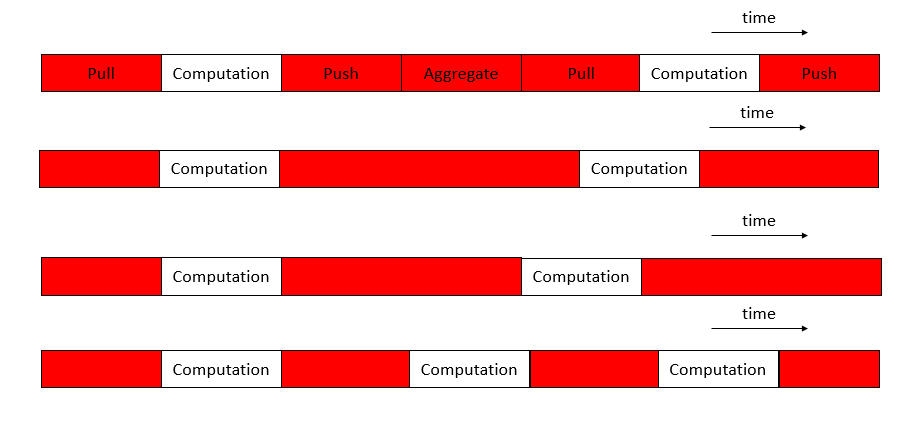
\includegraphics[scale=0.3]{figure/diffsizetime.png}
		\end{figure}
	\end{itemize}
\end{frame}

\subsection{Best size}
\begin{frame}
    \frametitle{Best size}
    \begin{figure}
		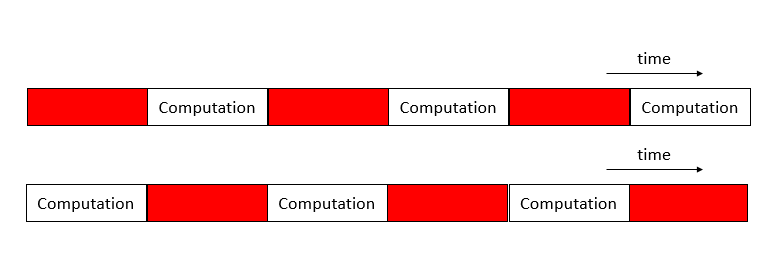
\includegraphics[scale=0.3]{figure/besttime.png}
	\end{figure}
\end{frame}

\subsection{Server view}
\begin{frame}
    \frametitle{Server view}
    \begin{figure}
		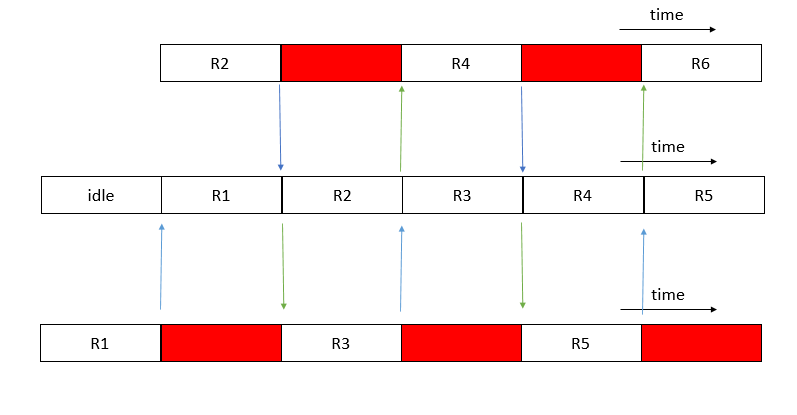
\includegraphics[scale=0.3]{figure/serverview.png}
	\end{figure}
\end{frame}



